\documentclass[11pt,dvipdfmx,b5paper,oneside,report]{jsbook}

\usepackage{color}
\usepackage{here}
\usepackage{framed}
\usepackage{tcolorbox}
\usepackage{quotchap}
\usepackage{pdfpages}
\usepackage[hidelinks]{hyperref}
\usepackage{pxjahyper}
\usepackage{titlesec}
\usepackage{picture}
\usepackage{tikz}
\usepackage{graphicx}
\usepackage{geometry}

\tcbuselibrary{breakable}
\definecolor{shadecolor}{gray}{0.80}



% section
\titleformat{\section}[block]{}{}{0pt}
{
  \definecolor{teal}{gray}{0.30}
  \begin{picture}(0,0)
    \put(-10,-5){
      \begin{tikzpicture}
        \fill[teal] (0pt,0pt) rectangle (5pt,19pt);
      \end{tikzpicture}
    }
    \put(-10,-5){
      \color{teal}
      \line(1,0){\hsize}
    }
  \end{picture}
  \hspace{0pt}
  \sf \Large \thesection
  \hspace{0pt}
}

% 図表見出し
\renewcommand{\tablename}{\textcolor{gray}{▼} 表}
\renewcommand{\figurename}{\textcolor{gray}{▲} 図}

\begin{document}

\begin{titlepage}
  \newgeometry{left=0cm,right=0cm,top=0cm,bottom=0cm}
  \centering
  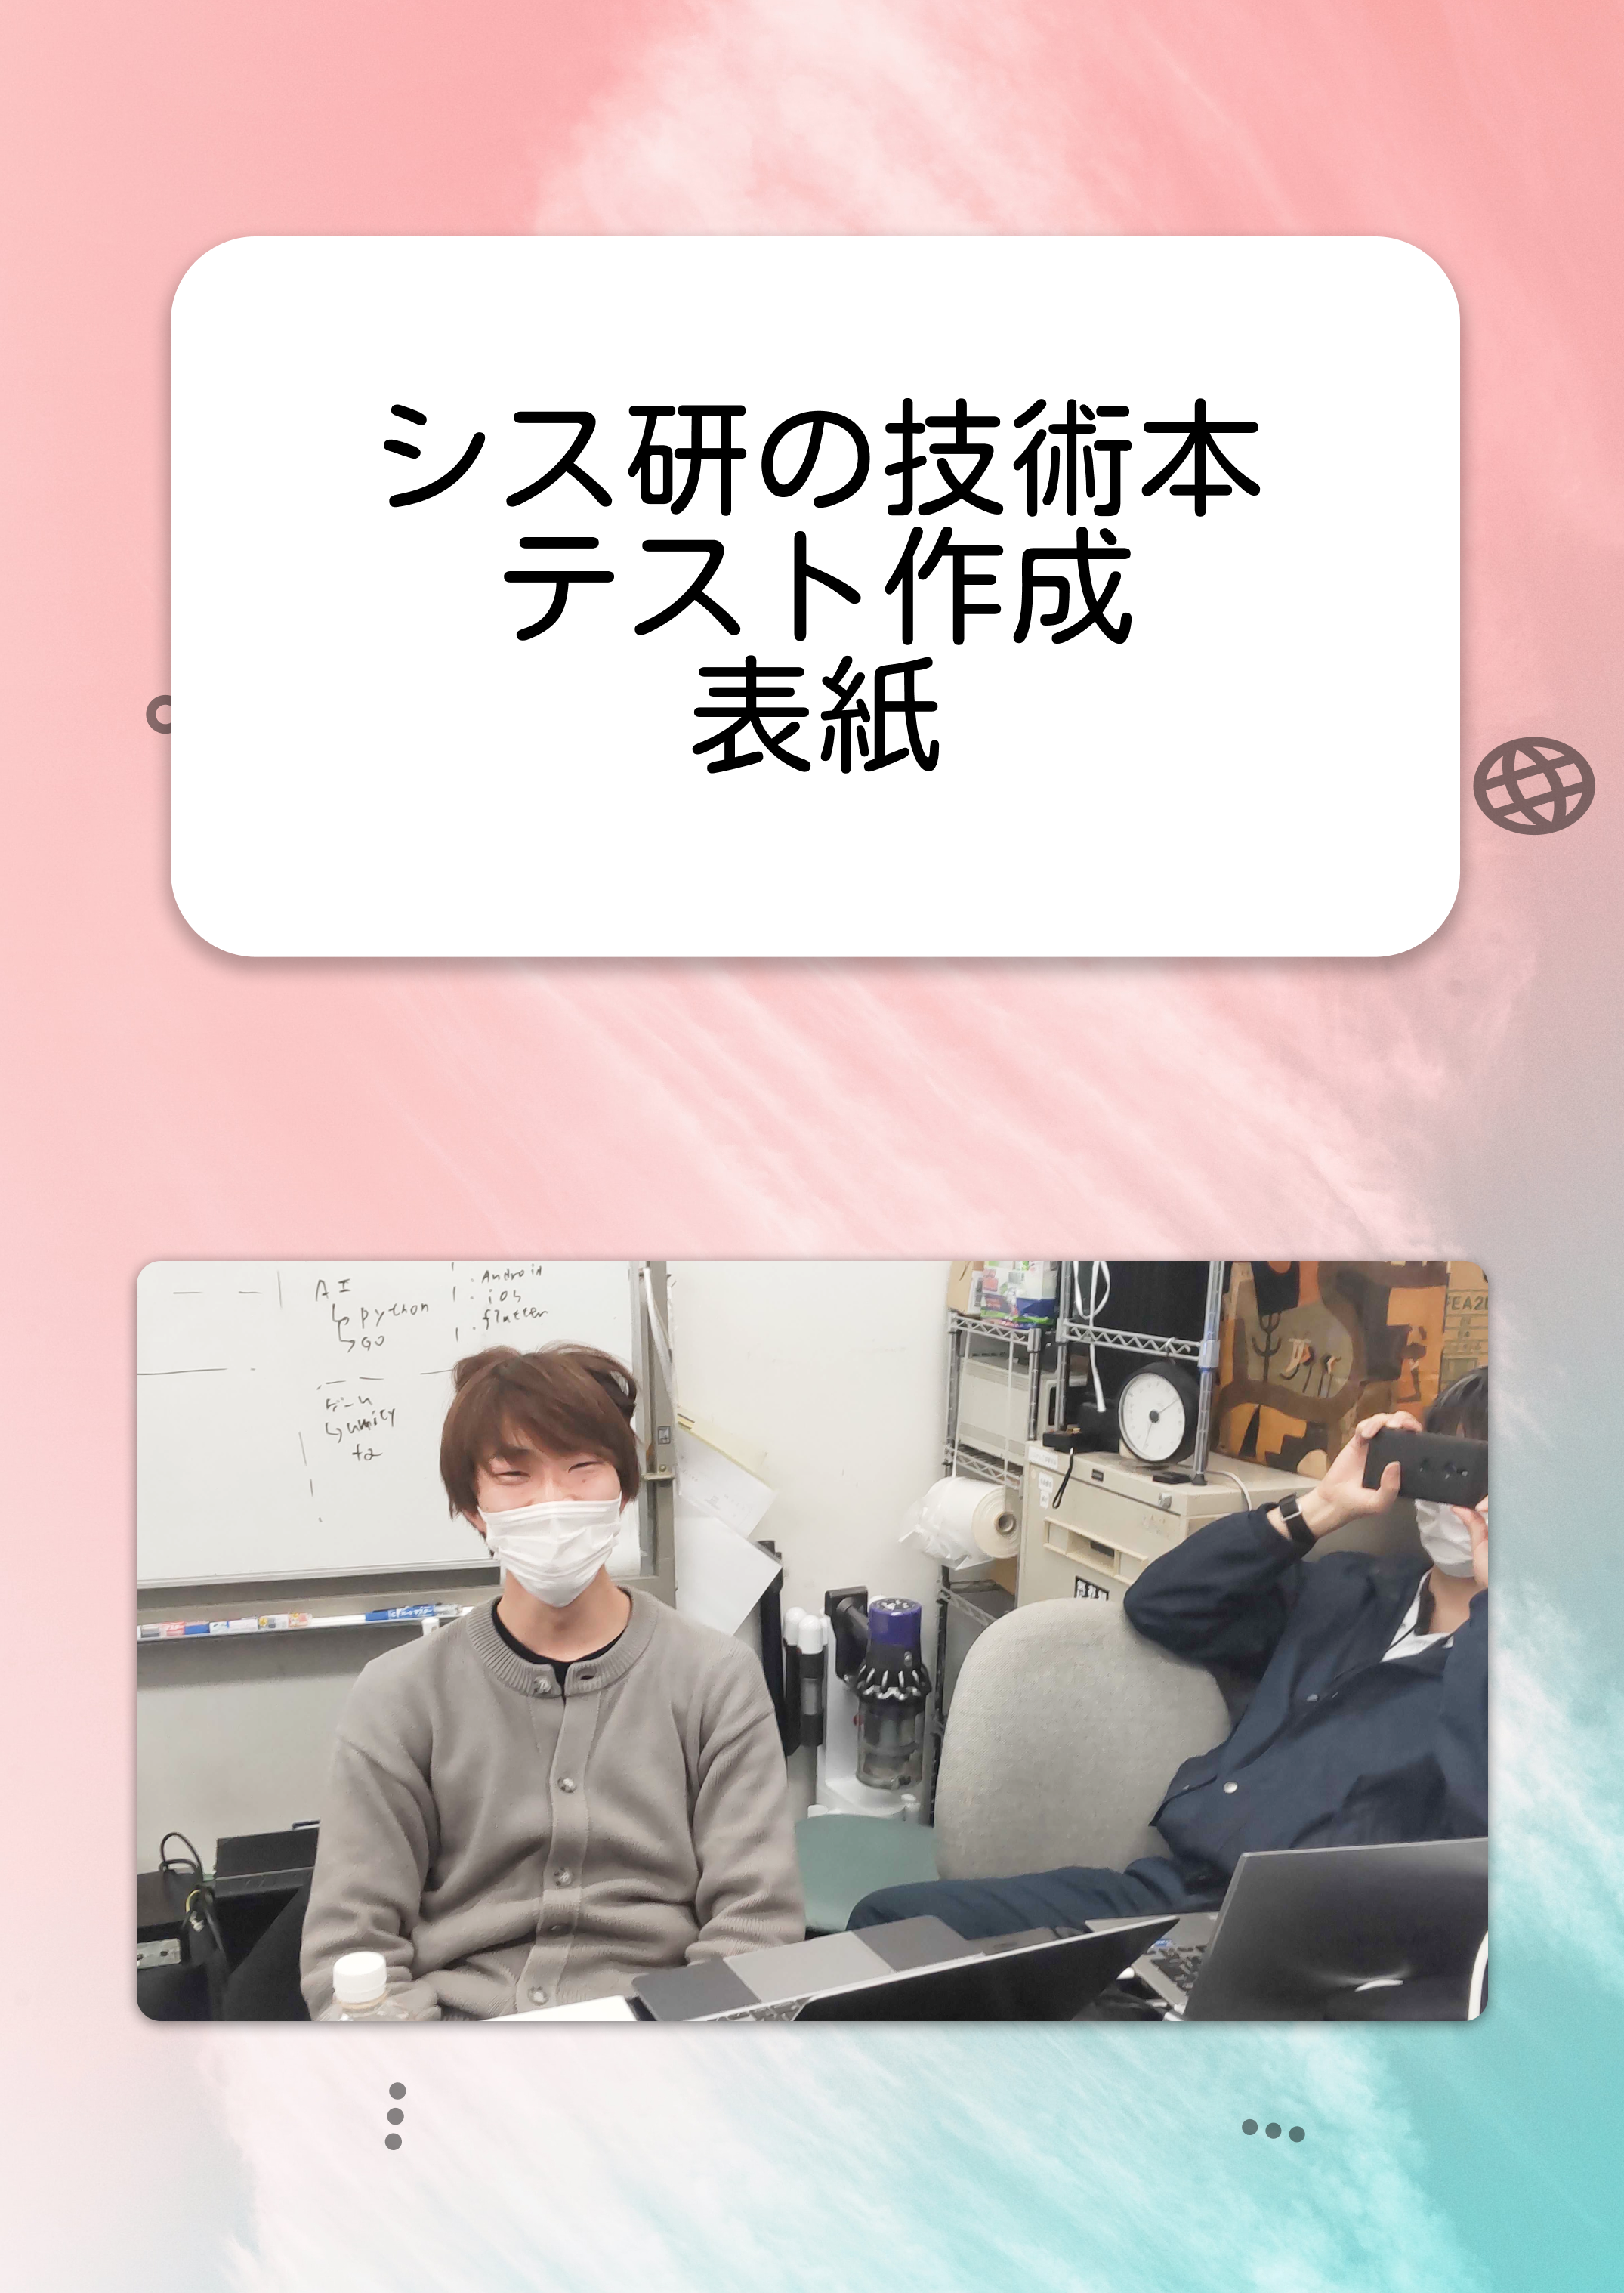
\includegraphics[width=\paperwidth,height=\paperheight]{image/titlepage.png}
  \restoregeometry % 元の余白に戻す
\end{titlepage}

%目次を自動的に作る。
\tableofcontents

\chapter{シス研の日常}

シス研は技術一辺倒ではなく、次のような活動をしているメンバーもいます!

\begin{tcolorbox}[title=お品書き]
  \begin{itemize}
    \item p.47『戦闘機に乗ろう』松土
          戦闘機のフライトシュミレータの紹介をしています!
  \end{itemize} 
\end{tcolorbox}

\begin{figure}[H]
  \centering
  \includegraphics[width=6cm]{./image/04-Intarasting/takoyaki_soryusyon.jpg}
  \caption{たこ焼きでITをそりゅーしょんしている様子}
  \label{takoyaki_soryusyon}
\end{figure}
\chapter{リポジトリ作成後に設定しておきたいこと}
\section{はじめに}
こんにちは。hihumikanです。

本チャプターでは「リポジトリ作成後に設定しておきたいこと」をご紹介します。
私自身が次回プロジェクト開始する際に、こういった設定をするだろうというものをまとめました。

ただし、これら全ての内容をプロジェクトに適用出来るものではないため、ご利用の環境や用途に合わせて利用していただければと思います。

\subsection{対象読者}

対象読者は、Git/GitHubを利用した開発を行う初学者の方を想定しています。

\section{ファイルの設定}

リポジトリ作成後に設定しておきたい「ファイルの設定」についてご紹介します。

\subsection{.gitignore}

.gitignoreは、Gitによる管理から除外したいファイルやディレクトリを指定するための設定ファイルです。

例えば、MacOSの場合、ディレクトリ毎に.DS\_Storeというファイルが自動的に生成されます。
このファイルは、ディレクトリのmeta情報を記録しますが、通常の開発において共有する必要がないため、Gitの管理対象外としておくことが望ましいです。

また、.envなどの環境変数を利用してプログラムを動かす場合、.envファイルには、パスワードや秘密鍵などの情報が含まれていることが多いため、これもGitの管理対象外としておくことが望ましいです。

リスト1.1のようなテキストファイルをGitの管理下に置くだけで、Gitから管理対象外として扱うことができます。

\begin{tcolorbox}[title=リスト1.1 .gitignore]
  \begin{verbatim}
1 .DS_Store
2 .env
\end{verbatim}
\end{tcolorbox}

リポジトリを共有する場合、.gitignoreファイルを共有することで、開発メンバー全員が同じ設定を利用できるため、必要なファイルだけがGitの管理下に置かれるようになります。

\subsection{.gitattributes}

.gitattributesは、特定のファイルに対してGitの挙動を変更するための設定ファイルです。
主に、改行コードやファイルの文字コードを指定することが多いです。改行コードの指定は、Windows(CRLF)とLinux(LF)の違いを吸収するために行います。


\subsection{Makefile}


\section{インフラ回り}

\subsection{GitHub Actions}
\subsection{renovate}
\subsection{webhooks}


\section{おわりに}
本チャプターでは「リポジトリ作成後に設定しておきたいこと」をご紹介しました。

\section{参考文献}
\begin{itemize}
  \item \href{https://git-scm.com/docs/gitignore}{gitignore}
  \item \href{https://git-scm.com/docs/gitattributes}{gitattributes}
\end{itemize}



\end{document}